\section{基于互信息和局部结构融合的 GRN 结构推断方法}
\label{sec:locpcacmi}

\subsection{引言}

从基因表达数据中推断基因调控网络 (GRNs) 的结构一直是系统生物学中的十分具有挑战的问题。
鉴定基因之间复杂的调控关系对于理解细胞的调控机制至关重要。
到如今,不少基于信息理论的 GRN 构建方法已经被提出来。
在上一章里面, 我们回顾了各种网络模型和建模方法。
基于信息理论的 GRN 推断方法属于关联网络建模方法的范畴。
然而,在传统的 DNA 微阵列测序数据中由于存在的外部噪声、
网络结构中的拓扑稀疏性和基因之间的传递依赖等因素,
使得基于信息理论的 GRN 推断方法在网络推断中会引入假阳性的依赖关系。
特别是随着网络规模的增加,这类方法的表现会大幅下降。
在本章,我们提出了一种新的网络结构推断方法 Loc-PCA-CMI。
该方法首先识别局部重叠基因簇 (local overlapped gene clusters),
然后基于条件互信息 (PCA-CMI) 的路径一致性算法推断每个簇的局部网络结构,
最终通过聚合局部网络结构,也就是基因之间的依赖性网络,来构建最终的 GRN。
我们在 DREAM3 敲除数据集上对 Loc-PCA-CMI 方法进行了评估,
将该方法与其它基于信息理论的网络结构推断方法,包括 ARACNE、MRNET、PCA-CMI 和 PCA-PMI,进行了比较。
实验结果证明, Loc-PCA-CMI 在 DREAM3 数据集上特别是在基因数目为 50 和 100 的网络上表现优于其它四种方法。

\subsection{相关工作}
\label{subsec:relatedwork}

推断和理解 GRNs 是系统生物学中的一个关键问题, 
可以帮助生物医学科学家明确识别基因与基因之间复杂的调控关系、理解细胞中的调控机制 \upcite{altay2010inferring, basso2005reverse}。
在过去, GRN 是从扰动或者敲除实验中推断出来的,然后对基因之间的调控相互作用进行二次验证。
显然,这种方法针对规模稍微偏大的基因集的调控关系推断是不可行的 \upcite{elnitski2006locating},需要耗费大量时间和相当大的成本。
由于微阵列技术的发展,大量的基因表达数据通过测序被得到,这使得基于计算方法从这些表达数据中推断出 GRN 成为可能 \upcite{maetschke2013supervised}。
% 近年来,基于计算方法的网络推断已成为最重要的目标之一 \upcite{altay2010inferring, margolin2006reverse}。
% 已经提出了各种用于GRN推断的方法,例如基于回归的方法 \upcite{Huynh-Thu2010, Haury2012, Huynh-Thu2014, liu2014group, li2017mgt, zheng2018bixgboost},
% 基于微分方程的方法 \upcite{sakamoto2001inferring, chowdhury2015stochastic, li2011large},
% 贝叶斯和动态贝叶斯网络 \upcite{murphy1999modelling, zou2004new, vinh2011globalmit, young2014fast, Liu2016, omranian2016gene},
% 以及基于状态空间的方法 \upcite{wu2003modeling, quach2007estimating}。
% 不幸的是,

% 基因表达数据通常具有高维度和相对较小的样本量,存在``维度诅咒"的问题 \upcite{wang2006inferring}。
% 此外,基因表达数据通常涉及大量外部噪声和非线性关系。
% 所有这些问题使得准确推断基因之间的调控相互作用,
% 尤其是在后基因组时代处理大规模基因表达数据时,
% 变得更加复杂和具有挑战性。

研究者基于各种不同的假设和不同的条件提出了从表达数据构建 GRN 精确结构的各种不同的计算方法 \upcite{longabaugh2005computational,karlebach2008modelling}。
目前的这些方法可以大致分为基于模型 (model-based) 和无模型 (model-free) 两大类别。

基于模型的方法通常制定系统的计算模型并进一步学习计算这些模型内部的参数。
典型的计算模型包括布尔网络 \upcite{shmulevich2002probabilistic,kim2007boolean,bornholdt2008boolean,zhou2016relative},
贝叶斯网络 \upcite{kim2003inferring,zou2004new,chen2006effective,needham2007primer,lo2015high},
以及微分方程模型 \upcite{gardner2003inferring,di2005chemogenomic,bansal2006inference, honkela2010model,lu2011high,li2011large}。
这些基于模型的方法的细节在上一章中有详细介绍, 因此我们不再重点介绍。
接下来, 我们转而介绍基于无模型 (model-free) 的方法。
% 布尔网络模型是最简单的网络模型,它通过布尔变量和布尔逻辑实现。
% 因为基因表达的状态被认为只是活动或非活动,布尔网络模型不能完全捕获复杂的系统行为 \upcite{lee2009computational}。
% 贝叶斯网络模型是一种流行的概率图形模型,其中基因之间的依赖关系通过有向无环图描述。
% 贝叶斯网络模型在处理噪声和结合先验知识方面优于其它模型,
% 但该模型中的结构学习是计算密集型的,并且已被证明是 NP 难问题 \upcite{chickering2004large}。
% 微分方程模型通过函数表征基因在特定时间的表达水平,其涉及与其它基因的调控相互作用。
% 通常,它将一个基因表达的变化率 (导数) 作为其它相关基因表达水平的函数。
% 使用微分方程模型重建 GRN 的一个主要挑战是如何在高维模型中有效识别模型结构和估计参数。
% 关于各种数据驱动建模方案和相关主题的文章评论,可以参考 \upcite{hecker2009gene,marbach2012wisdom,wu2007inference,liu2012reverse,li2018control}。

基于无模型 (model-free) 的方法主要通过衡量基因之间的依赖性来识别调控相互作用,
典型的算法包括基于相关性和基于信息理论的方法。
在基于相关性的方法中,调控相互作用由两个基因之间的共表达程度决定,
例如 Pearson 相关性,秩相关性,欧几里德距离和表达值向量之间的角度 \upcite{wang2014review}。
然而,基于相关性的方法无法识别基因之间的复杂依赖性,例如非线性依赖性 \upcite{ruyssinck2014nimefi}。
此外,相当多的功能相关的基因, 比如管家基因,可能不会共表达,因此难以准确推断它们之间的调控相互作用。
基于信息理论的方法也是一种代表性的无模型 (model-free) 方法。
信息理论在测量两个变量之间的非线性依赖关系时相对高效, 
因此越来越多地用于衡量基因间的调控关系强弱,其中互信息和条件互信息应用最为广泛。
其中互信息 (MI) 有助于衡量基因之间的潜在依赖性,
因为它可以有效地捕获非线性依赖关系 \upcite{brunel2010miss,zhang2011inferring}。
近年来,研究者陆续提出了基于信息理论的各种网络推断方法,
其侧重于区分调控中的直接相互作用和间接相互作用 \upcite{marbach2010revealing}。
互信息 (MI) 的定义如下:
\begin{align} % requires amsmath; align* for no eq. number
    MI(X,Y)=\int \int p(x,y)log \frac{p(x,y)}{p(x)p(y)}dxdy
 \end{align}
 其中 $p(x,y)$ 表示两个变量 $X$ 和 $Y$ 的联合概率密度函数。
 $X$ 是基因表达量数据,其中的元素表示不同条件 (样本) 中相应基因的表达值。
 $p(x)$ (或者 $p(y)$) 表示 $X$ (或者 $Y$ )的边缘概率密度分布。

条件互信息 (CMI) 可以用熵表示为:
\begin{equation}
\begin{split}
CMI(X,Y|Z) &= H(X,Z) + H(Y,Z)\\
               & - H(Z) - H(X,Y,Z)
\end{split}
\end{equation}
其中 $H(X,Z)$, $H(Y,Z)$, $H(X,Y,Z)$ 表示联合熵。
CMI 值越高,表明给定变量 $Z$ ,变量 $X$ 和 $Y$ 之间越可能存在密切关系。

熵可以用高斯核概率密度来估计 \upcite{basso2005reverse},变量 $X$ 的熵可以通过如下方式计算, 
其中 $|C|$ 是变量 $X$ 协方差矩阵的行列式 \upcite{zhang2011inferring}:
\begin{equation}
    H(X) = log(2\pi e )^\frac{n}{2} |C| ^ {-\frac{1}{2}}
\end{equation}

进一步地,我们可以得到下面的等式 \upcite{zhang2011inferring}:
\begin{equation}
    MI(X,Y)=\frac{1}{2}log\frac{|C(X)|*|C(Y)|}{|C(X,Y)|}
\end{equation}

Margolin 等人 \upcite{margolin2006aracne}提出了 ARACNE 方法,使用数据处理不等式 (DPI) 来过滤掉来自三重基因的间接相互作用。
Meyer \upcite{meyer2007information} 的最小冗余网络 (MRNET) 使用最小冗余特征选择方法 \upcite{peng2005feature},
其中对于网络中的每个候选基因,它选择其高度相关基因的子集, 同时最小化所选基因之间基于互信息的相关性。
Zhang 等人 \upcite{zhang2011inferring} 介绍了一种基于条件互信息的路径一致性算法 PCA-CMI ; 
Zhao 等人 \upcite{zhao2016part} 引入了基于偏互信息的路径一致性算法 PCA-PMI 。
下面我们将重点介绍 PCA-CMI 算法,PCA-PMI 算法的思路与之类似。

PCA-CMI 算法利用 MI 和 CMI,从低阶到高阶递归地移除基因调控网络中具有独立或条件独立关系的边, 具体的步骤如下:

步骤 0:初始化。输入基因的表达数据 $M$, 设置阈值参数 $\beta$, 用来判断是否满足独立性。
选择所有的基因建立全连通网络, 设置 $L=-1$。

步骤 1:$L=L+1$, 对于非零边, $G(i,j) \neq 0$, 选择同时与基因 $i$ 和基因 $j$ 相连接的邻近基因, 
假定这些基因 (不包括基因 $i$ 和基因 $j$ ) 的数量为 T。

步骤 2:如果 $T<L$, 停止。如果 $T>L$, 从这 $T$ 个基因中选取 $L$ 个基因, 
并把它们表示为 $K=[k_1,\ldots,k_L]$。
对于 $K$, 可选择的数目为 $C_T^L$。
对于所有的 $C_T^L$ 种 K ,选择计算出 $L$ 阶 $CMI(x,j|K)$,
并选择出最大的一个标记为 $I_{max}(x,j|K)$。
如果 $I_{max}(x,j|K) < \beta$, 设定 $G(i,j)=0$, 并返回到步骤 1 中。

从上述步骤可以看出, PCA-CMI 是一种采用了 top-down 策略的算法, 
从全通图中不断寻找子图, 在每个子图结构里按照 CMI 的独立性阈值条件来删减边,直至满足临界条件。
显然, 在这个算法里面独立性阈值 $\beta$ 是全局变量, 需要依靠先验知识来获取合适的值。

路径一致性算法 (Path Consistency Algorithm, PCA) 是一种穷举算法,广泛用于推断 GRN \upcite{zhang2011inferring}。
PCA-CMI 和 PCA-PMI 这两个算法通常会在运行时间和准确度之间进行折衷权衡。
值得注意的是, 
随着网络规模的增加, 网络噪声在增加,
PCA 这种 top-down 的算法的复杂度很高, 而且受到经验参数的影响,使得 GRN 的预测精度急剧下降。

\subsection{GRN 结构推断方法}
为了改善 PCA 在随着网络规模增加复杂度变高, GRN 预测精度急剧下降的状况,我们直接从局部结构入手,辅助以合并的策略,提出了一种新的基因调控网络结构推断方法,命名为 Loc-PCA-CMI。
该方法首先使用高度共同表达的基因作为局部基因簇的质心,
然后使用 PCA-CMI 对每个簇的结构进行构建, GRN 的最终结构是将所有局部网络结构进行合并。
从这个流程可以看出, Loc-PCA-CMI 方法可以处理相对较大的数据集,
并且将从 PCA-CMI 在小规模基因子网的相对准确的结构推断上受益。
接下来,我们将重点介绍我们提出的 GRN 结构推断方法 Loc-PCA-CMI 以及 Loc-PCA-PMI。

\subsubsection{算法 Loc-PCA-CMI}

众所周知,生物系统中节点之间是很少完全连通的,
大多数节点只直接连接到少量其它节点 \upcite{jeong2000large},因此 GRN 也是一种稀疏网络。
识别网络的稀疏结构的关键步骤是识别可能具有相对高的共表达值的边。
具体来说,我们提出的 Loc-PCA-CMI 首先通过 Pearson 相关性分析和 $p$ 值错误率 (FDR) 校正选择 top $n$ 条高度共表达的边;
然后,在缩减的边构成的空间中,用边连接的基因计算局部重叠基因簇。
然后对于每个局部基因簇, 我们应用 PCA-CMI 算法 \upcite{zhang2011inferring},
它可以通过从低到高依赖关联重复去除不相关的边来构建高置信度无向网络 \upcite{spirtes2000causation},
直到没有边可以删除,从而获取到每个局部网络的最终结构 (见 \ref{subsec:relatedwork})。
最后, 我们对每个推断的局部子网络结构边权重取平均,来获得完整的调控网络的边的权重。
整个方法流程如图 \ref{pca-cmi-fr} 所示,实现细节如算法 \ref{alg} 所示。
需要注意的是,
在算法 \ref{alg} 里面,
由于 PCA-CMI 本身就非常适合相对较小的 GRN 结构推断,
因此我们设置了一个过滤预处理步骤: 如果局部网络中基因的数量小于或等于常数 $c$,
则直接应用 PCA-CMI 推断其对应的 GRN 的结构。
\begin{figure}[!htbp]
    \centering
    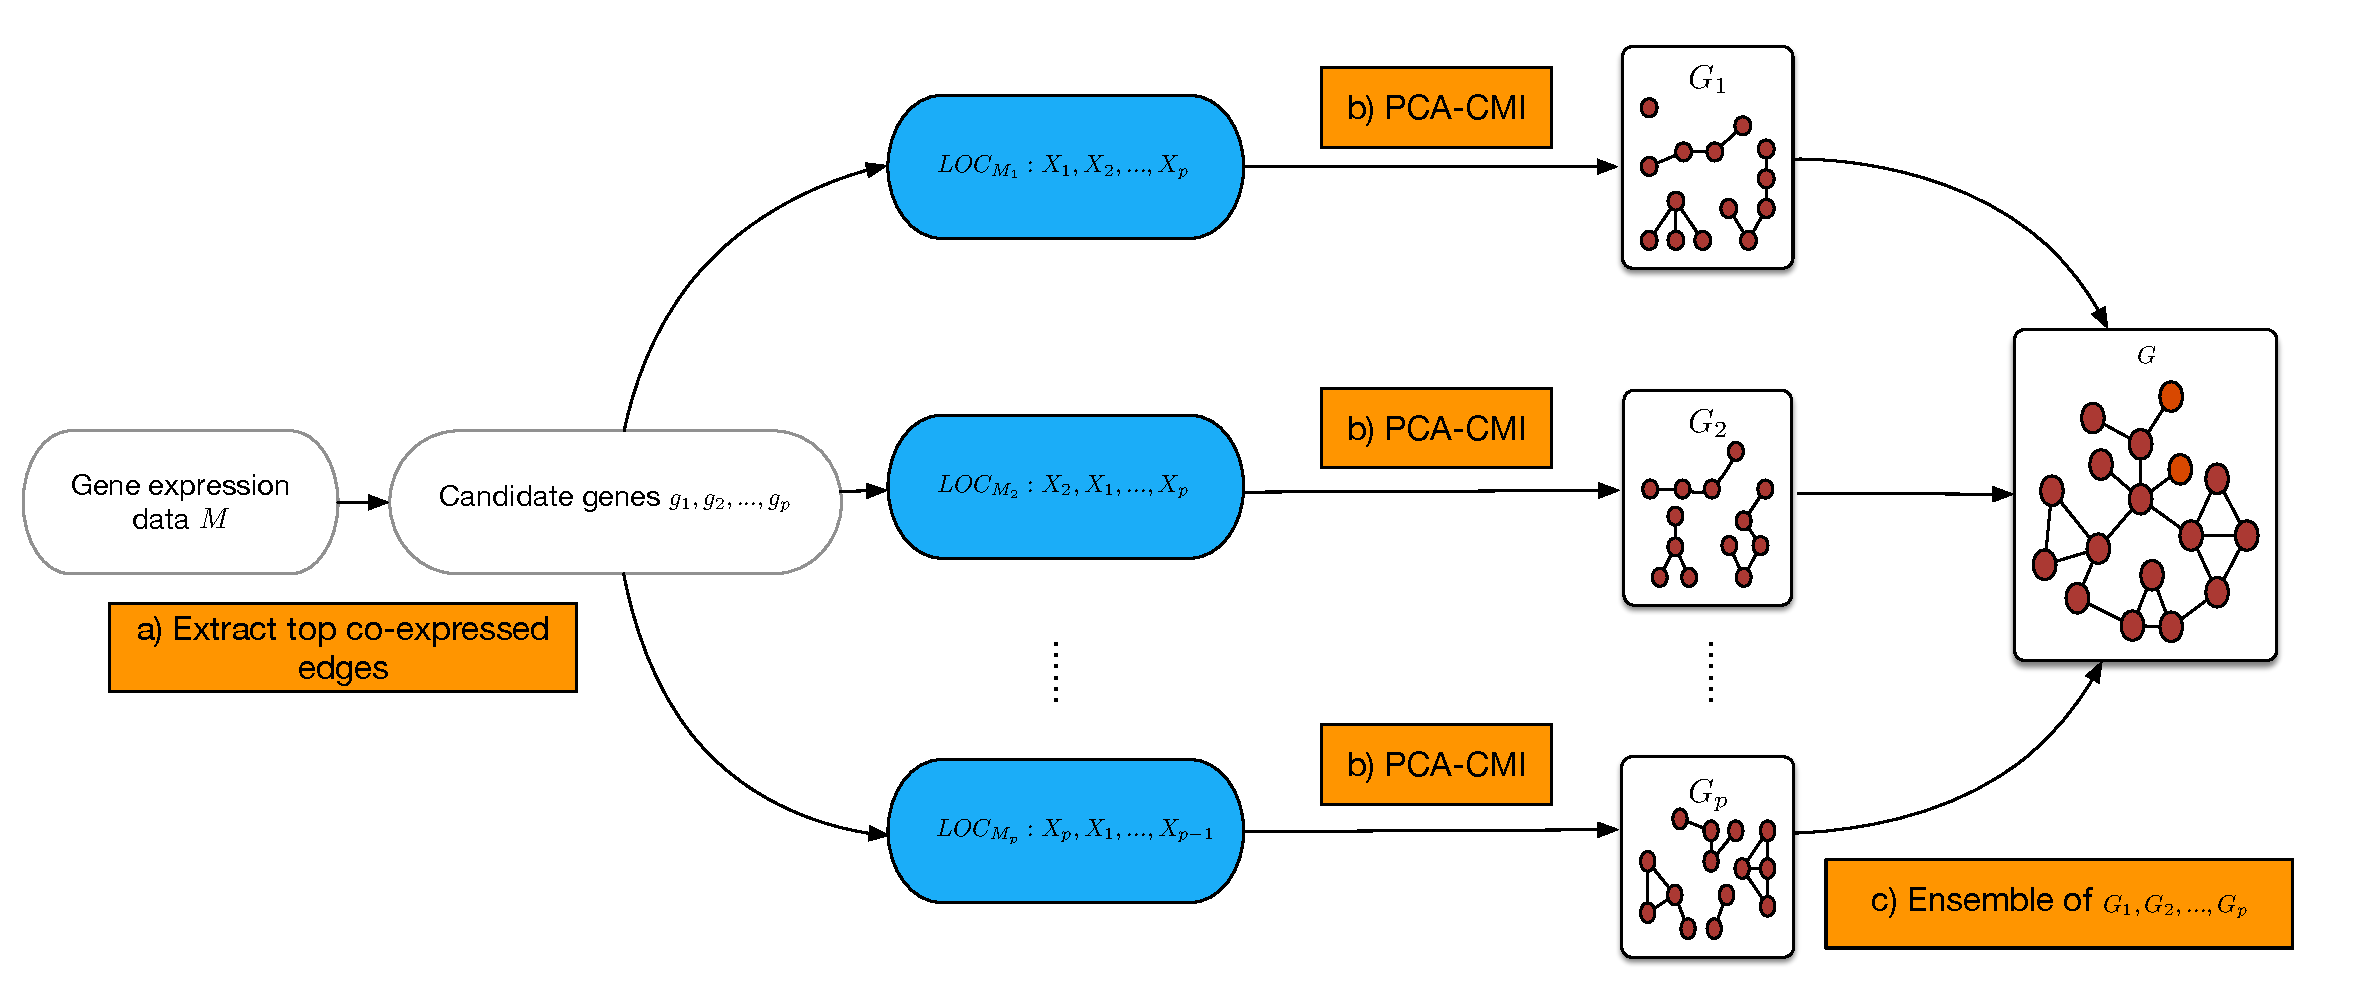
\includegraphics[width=0.95\textwidth]{pca-cmi-framework.pdf}
    \caption{Loc-PCA-CMI 方法框架图。
    (a) 从基因表达矩阵 $M$ 中抽取 top $n$ 条共表达边,其对应的候选基因为 $g_1,g_2,\ldots,g_{p} $。
    这些候选基因被分组到局部簇中 $LOC_{M_1}, LOC_{M_2},\ldots,LOC_{M_{p}}$,
    其中 $g_1,g_2,\ldots,g_{p}$ 是分别作为每个簇的质心。
    (b) 对每一个局部之间有重叠的簇,我们应用 PCA-CMI 算法来得到它准确的结构。
    (c) 聚合 $G_1, G_2, \ldots, G_p$ 来得到 GRN 的最终结构图 $G$。
    }
    \label{pca-cmi-fr}
\end{figure}

\begin{algorithm}[!htbp]
    \caption{Loc-PCA-CMI 算法伪代码}
    \label{alg}
    \begin{algorithmic}[1]
    \Require $M$ (the gene expression data matrix), $m$ (the number of genes), $n$ (the number of top ranked edges), $c$ (constant number); $k$ (CMI order number) and $\beta$ (order threshold) in subroutine PCA-CMI.
    \Ensure Graph weight matrix $G$ 
    \If {$m \leq c$} 
    \State $G$ $\leftarrow$ PCA-CMI$(M, k, \beta)$;
    \State \Return $G$
    \Else
    \State Construct pair-wise gene-gene Pearson correlation matrix $\Omega = \rho(M_i, M_j)$;
    \State Select top $n$ edges as $E$ with highest Pearson correlation value in $\Omega$ with FDR correction in p-value, and according to which to get 
    $p$ candidate genes as $g_1,g_2,\ldots,g_{p}$;
    \For{each gene in $g_1,g_2,\ldots,g_{p}$} 
      \State Retrieve its directly connected genes that in edges list $E$ as local cluster $LOC_{M_i}$;
    \EndFor
    \For{each cluster $LOC_{M_i}$  in $LOC$}
      \State $G_{i}$ $\leftarrow$ PCA-CMI$(LOC_{M_i}, k, \beta)$;
    \EndFor
    \State $G$ $\leftarrow$ mean$(G_{1},G_{2},\ldots,G_{p})$;
    \State \Return $G$ \Comment{Return the graph weight matrix}
    \EndIf
    \end{algorithmic}
\end{algorithm}

算法 \ref{alg} 的计算复杂度由两个因素决定:
 第一个是局部重叠基因簇 $p$ 的数量,通常低于基因的总体数目 $m$; 
第二个是 PCA-CMI 子程序本身的算法复杂度。
 PCA-CMI 的计算复杂度由 CMI 阶数 $k$ 和 $LOC_{M_i}$ 的簇大小 $|C|$ 控制,
可以粗略估计为 $O(|C|^k)$。
因此, PCA-CMI 的最终算法复杂度为 $O(m *|C|^k)$。
在最坏的情况下, 如果簇大小 $|C|$ 等于 $m$, 也就是每个簇包含其中的所有基因, 
那么计算复杂度为 $m*m^k = m^{k+1}$。 
然而,这种最糟糕的情况在实验中很少发生,因为 $|C|$ 通常低于 $m$。
另外,在实际实验过程中,所有 PCA-CMI 子程序可以并行执行, Loc-PCA-CMI 能以很快的速度执行完毕。

\subsubsection{算法 Loc-PCA-PMI }

在算法 \ref{alg} 中,获得每个局部基因簇之后,
 PCA-CMI 和 PCA-PMI 都可以视为后续局部结构推断的候选方法。
如果在局部结构构建时使用 PCA-PMI 替换 PCA-CMI,我们将该方法命名为 Loc-PCA-PMI。
其对应的方法框架如图 \ref{pca-pmi-fr} 所示, 
 Loc-PCA-PMI 与 Loc-PCA-CMI 唯一不同的地方在局部网络结构构建的时候 (如图 \ref{pca-pmi-fr} 中虚线部分所示),
 Loc-PCA-PMI 的实现细节在这里不再赘述了,感兴趣的读者可以参考算法 \ref{alg} 自行推理出来。
同样地,由于子程序 PCA-PMI 跟 PCA-CMI 的算法复杂度相同,
因此, Loc-PCA-PMI 的计算复杂度跟 Loc-PCA-CMI 保持一致。

\begin{figure}[!htbp]
  \centering
  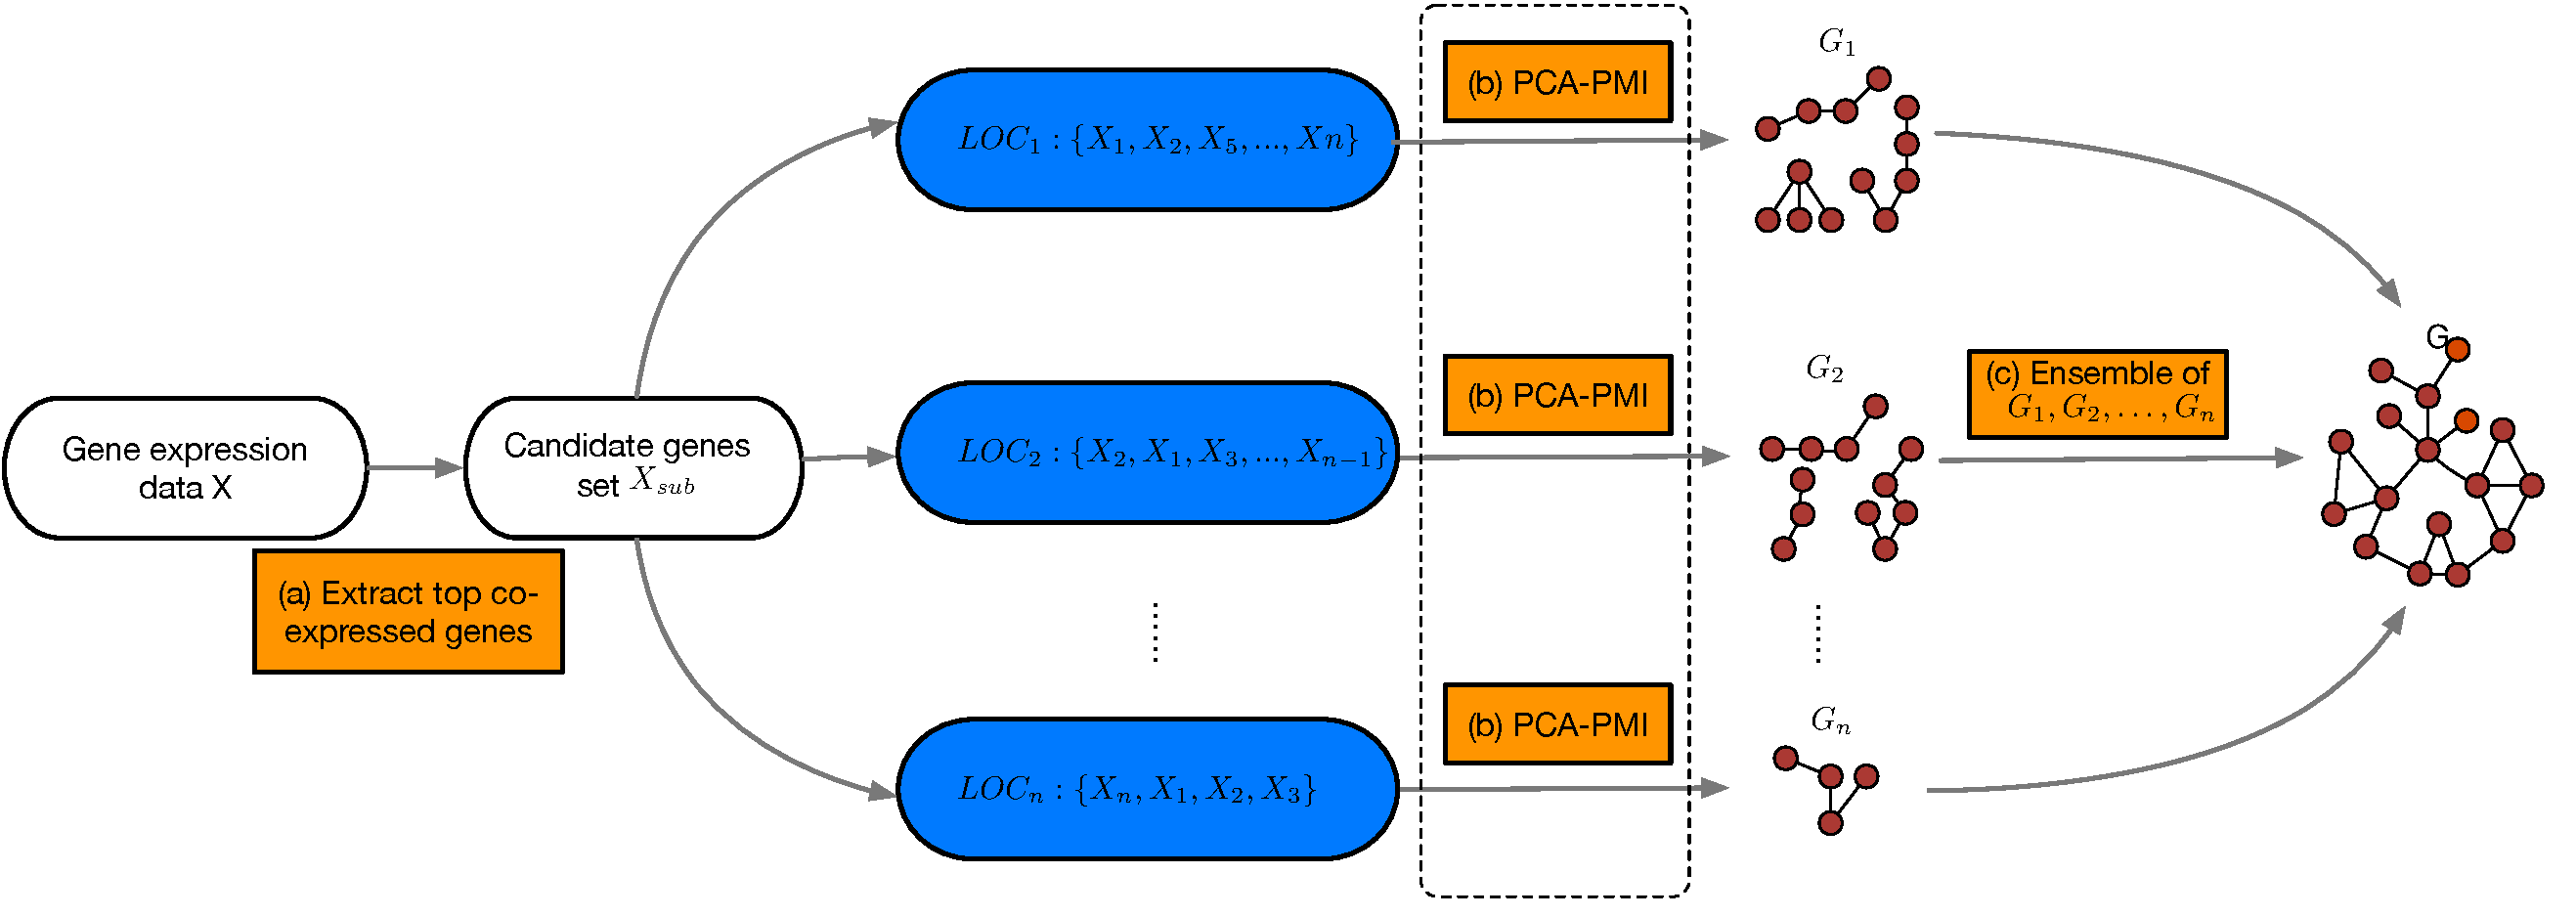
\includegraphics[width=0.95\textwidth]{pca-pmi-framework.pdf}
  \caption{Loc-PCA-PMI 方法框架图。算法流程与 Loc-PCA-CMI 方法类似。}
  \label{pca-pmi-fr}
\end{figure}

% 综合上文,我们的讨论涉及到了四种基于路径一致性的方法,即是 PCA-PMI、PCA-CMI、Loc-PCA-PMI 和 Loc-PCA-CMI。

\subsection{实验结果}

\subsubsection{数据集}

在过去十年中, GRN 推理一直是一个相当活跃的研究领域。
因此,一个英文译名为``逆向工程对话"的社区联盟 (DREAM) \upcite{stolovitzky2007dialogue} 成立。
由该组织举办的 DREAM Challenge 是生物医药领域最具影响力的开放数据建模旗舰竞赛,
旨在通过算法解决当前热点的生物学问题。
该赛事根据当下热点的研究问题发起挑战竞赛,由组织方提供测试数据,
并设计不同的任务主题供参赛者进行建模预测,根据预测结果决定优胜者。
其第三方验证的特性保证了算法的可重复性,使得算法能得到最有效的验证,
从而在推动在该研究领域的进展。
目前该赛事已经完成了 50 多项挑战赛,产生了近百篇相关的文献。

DREAM 联盟举办了 DREAM3、
DREAM4 和 DREAM5 等与 GRNs 推理构建相关的挑战赛, 
举办方提供了标准化的通用输入数据集和性能评估指标来比较不同的候选方法。
该组织提供的数据集事实上成为了 GRN 推理领域的金标准网络数据集,
经常被用于评测各种各样新的 GRN 构建算法。

本章使用来自 DREAM3 挑战赛的六个模拟数据 \upcite{schaffter2011genenetweaver} 对 Loc-PCA-CMI 的性能进行了测试。
 DREAM3 使用 GeneNetWeaver 软件来模拟生成基因网络表达数据,
在来自已知生物模式的调节相互作用系统的子网:
 Ecoli (大肠杆菌) 和 Yeast (酵母) 的基础上,得到测试使用的基准网络。 
在实验中,我们采用了 DREAM3 中的总计六个基因敲除表达网络,
其包括三种不同规模的网络节点数:
 10、 50、 100, 和两种不同类型的生物: Ecoli 和 Yeast, 
来对所有的测试方法包括 Loc-PCA-CMI 进行评估。

表 \ref{tbl} 展示了这 6 个数据集的样本数目 (Number of samples)、节点平均 (最大)度 (Average(Max) degree)、边数目 (Number of edges) 和网络密度 (Network density)。
它们的节点平均度都在 2-3 之间, 网络密度随着节点数目增多而下降。

\begin{table} [!htbp]
  \caption{实验所使用的数据集描述} 
  \label{tbl} 
  \resizebox{\columnwidth}{!}{%
  \centering  
  \begin{threeparttable}  
  \begin{tabular} {cccccc} 
  \toprule
  Datasets  & Number of samples & Average(Max) degree & Number of edges & Network density \\ 
  \midrule
  DREAM3-10 Ecoli &11 & 2.2(5) & 11 & 0.244\\
  DREAM3-50 Ecoli & 51 & 2.48(14) & 62 & 0.051\\
  DREAM3-100 Ecoli & 101 & 2.5(14) & 125 & 0.025\\
  DREAM3-10 Yeast &11 & 2(4) & 10 & 0.222\\
  DREAM3-50 Yeast & 51 & 3.08(13) & 77 & 0.063\\
  DREAM3-100 Yeast & 101 & 3.32(10) & 166 & 0.034\\
  \bottomrule
  \end{tabular}
  \end{threeparttable}  
  }
\end{table} 

针对每个数据集而言,输入数据文件中的行代表样本 (实验),列代表基因 (实验变量)。
第一行是野生型表达数据,该样本中的每个基因都保持稳定状态。
第 $l$ ($l>1$) 行则表示在对应的样本中第 $l-1$ 个基因敲除后其它基因的表达量。
读者可以在 GitHub 仓库 \url{https://github.com/chenxofhit/Loc-PCA-CMI.git} 上查看我们在本章节实验用到的数据集。

\subsubsection{评价指标}

我们通过评估接收者操作特征曲线下面积 (AUROC) 和准确率召回率曲线下面积 (AUPR) 来评估 Loc-PCA-CMI 的性能。
与稀疏生物网络一样,不存在的边 (负样本) 的数量明显超过现有边 (正样本) 的数量; 
事实上, AUPR 对 AUROC 提供了更多信息 \upcite{saito2015precision} 。
本文倾向于使用 AUPR 进行评估,但为了与采用 AUROC 作为评估指标的其它方法进行完整地比较,
我们也计算了 AUROC 作为补充。
总体上来讲,较高的 AUROC 和 AUPR 值表明更准确的 GRN 预测。

为此,本文通过比较金标准网络 (golden network) 中的真实边与方法 Loc-PCA-CMI 输出的有序边列表里最高 $q$ 条边来计算真阳性 (TP)、真阴性 (TN)、假阳性 (FP) 和假阴性 (FN) 边的数量。
通过绘制真阳性率 (The true positive rates, TPR) 与假阳性率 (The false positive rates, FPR) ,
我们便得到了接收者操作特征 (Receiver Operating Characteristic, ROC) 曲线; 
同样地,
%The ROC curve is constructed by plotting the true positive rates (TPR = TP/(TP + FN)) versus the false positive rates (FPR = FP/(FP + TN)) for increasing $q$ ($q = 1,2,\ldots,m^2$).
精确率-召回率 (Precision-Recall, PR) 曲线是通过绘制精确率 Precision 与召回率 Recall 而得到。
其中, TPR、FPR、Precision、Recall 的计算分别如等式 \ref{eq:tpr}、\ref{eq:fpr}、\ref{eq:precision}、\ref{eq:recall} 所示。
我们再通过计算曲线下的面积便得到了 AUROC 和 AUPR。

\begin{equation}
  \label{eq:tpr}
  \text{TPR} = \frac{\text{TP}}{\text{TP + FN}}
\end{equation}
\begin{equation}
  \label{eq:fpr}
  \text{FPR} = \frac{\text{FP}}{\text{FP + TN}}
\end{equation}
\begin{equation}
  \label{eq:precision}
  \text{Precision} = \frac{\text{TP}}{\text{TP} + \text{FP}}
\end{equation}
\begin{equation}
  \label{eq:recall}
  \text{Recall} = \frac{\text{TP}}{\text{TP} + \text{FN}}
\end{equation}
\begin{equation}

\subsubsection{模型选择}
在算法 \ref{alg} 中总计有三个参数会影响方法 Loc-PCA-CMI 的性能。
第一个参数是选定的 top 边的数目 $n$,
如果 $n$ 增加,则考虑的共表达的边数目增大,局部基因簇的大小将增加。
第二个参数是 $\beta$,它作为 MI 和 CMI 的阈值来决定独立性。
第三个参数是 CMI 阶数 $k$,从理论上讲,通过增加 $k$,如果 CMI 没有达到 $k-1$ 阶的阈值 $\beta$,结构会更准确。
第二和第三这两个参数属于 PCA-CMI 和 PCA-PMI 方法里面的固有参数。
$n$ 的最佳值可以通过交叉验证获得,通常较大的 $n$ 可以促成使得每个子网络中涵盖更多的基因;
在实验中,我们将其值统一设置为 $n =\binom{m} {2}/5$。
除了上述三个参数外,我们在算法 \ref{alg} 中设置常量 $c = 10$,
即如果基因数小于或等于 10,则 Loc-PCA-CMI 直接调用 PCA-CMI,
显然在这种情况下, Loc-PCA-CMI 和 PCA-CMI 的性能是相同的。

% 如表 \ref{tbl} 所示,在六个基准数据集 DREAM3-10 中,因为 Ecoli 和 Yeast 数据集仅包含 10 个基因,
% 满足算法 \ref{alg} 的过滤预处理条件,
% 此时, Loc-PCA-CMI 和 PCA-CMI 在这两个数据集上的输出的调控网络结构相同,
% 同样地此时 Loc-PCA-PMI 和 PCA-PMI 输出的调控网络结构也相同。
% 为了对这些基于 PCA (路径一致性) 的方法进行更有意义的比较,
% 我们选择了其它四个基因数目大于 10 的数据集。

为了探讨阶数 $k$ 的大小是如何影响这些方法的性能,
按照文献 \upcite{zhang2011inferring,zhao2016part} 中建议的参数取值,
设置固定阈值 $\beta = 0.03$ 后,
我们把这四种方法中的阶数 $k$ 从 1 逐渐变化为 10,
然后分别计算每种方法的 AUROC 和 AUPR。
图 \ref{fig:k} 总结了它们在基准数据集上的实验结果, 
我们可以看出, 阶数 $k$ 会对这四种基于 PCA 的方法的结果产生影响,
通常当 $k$ 达到 4 时 AUPR 和 AUROC 变得稳定,除了 DREAM3-100 Ecoli 数据集上略有不同。

\begin{figure*}[!htbp]
    \centering
    \begin{minipage}[b]{0.45\linewidth}
      \centering
      \centerline{
        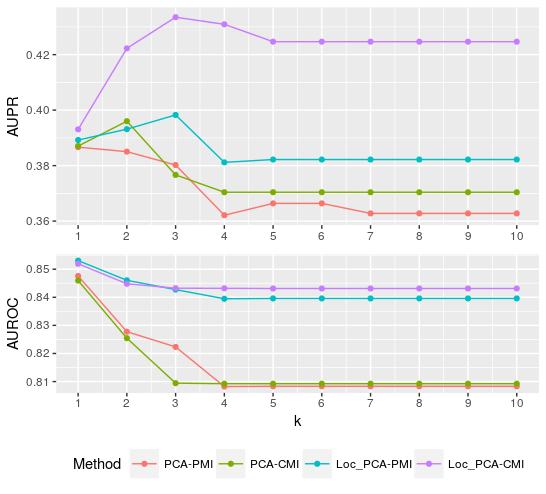
\includegraphics[width = \linewidth]{K_Dream50_Ecoli.png}}
      \centerline{(a) DREAM3-50 Ecoli}
      \medskip  
    \end{minipage}
    \begin{minipage}[b]{0.45\linewidth}
      \centering
      \centerline{
        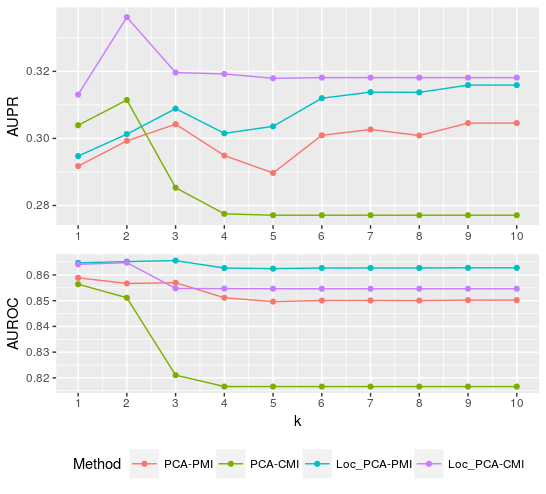
\includegraphics[width =\linewidth]{K_Dream100_Ecoli.png}}
      \centerline{(b) DREAM3-100 Ecoli}
      \medskip  
    \end{minipage}
      \begin{minipage}[b]{0.45\linewidth}
      \centering
      \centerline{
        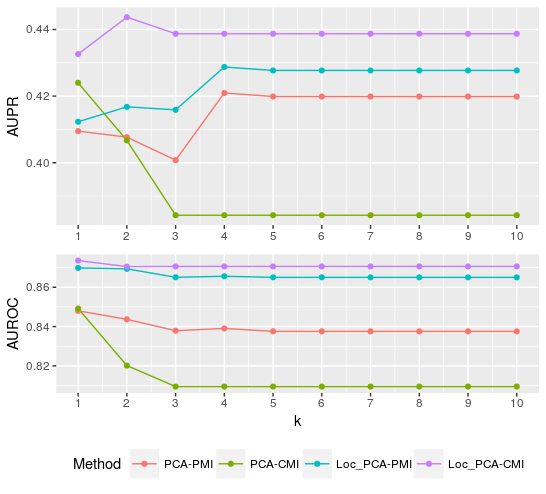
\includegraphics[width = \linewidth]{K_Dream50_Yeast.png}}
      \centerline{(c) DREAM3-50 Yeast}
      \medskip  
    \end{minipage}
    \begin{minipage}[b]{0.45\linewidth}
      \centering
      \centerline{
        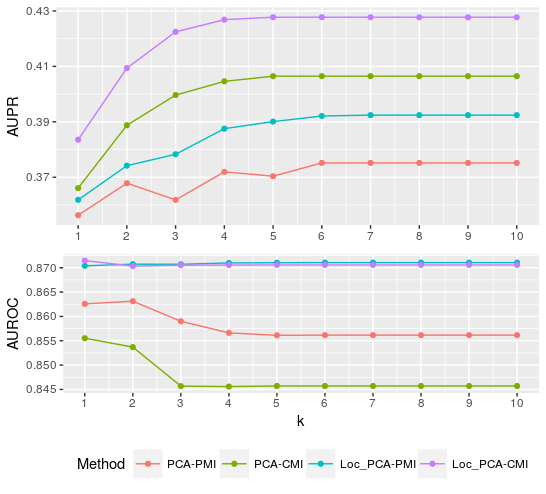
\includegraphics[width =\linewidth]{K_Dream100_Yeast.png}}
      \centerline{(d) DREAM3-100 Yeast}
      \medskip  
    \end{minipage}
    \caption{%AUPR and AUROC  by varying $k$ from 1 to 10 of four PCA based methods on four different datasets: 
    在四个不同的数据集上 k 值从 1 改变到 10, 基于路径一致性的四个算法的 AUPR 和 AUROC 结果示意图。
    }
    \label{fig:k}
\end{figure*}

固定阶数 $k = 2$ 后, 我们在 $\beta = [0.01,0.02,0.03,0.05,0.1,0.15,0.2]$ 上对这四种算法也进行了测试, 
分别计算出每种方法的 AUROC 和 AUPR。
图 \ref{fig:beta} 总结了它们在基准数据集上的结果, 
可以看出, 阈值独立性参数 $\beta$ 会对这四种基于 PCA 的方法的结果产生影响,
AUPR 总体上随着 $\beta$ 的增加逐渐增大,然后又逐渐降低。

\begin{figure*}[!htbp]
    \centering
    \begin{minipage}[b]{0.45\linewidth}
      \centering
      \centerline{
        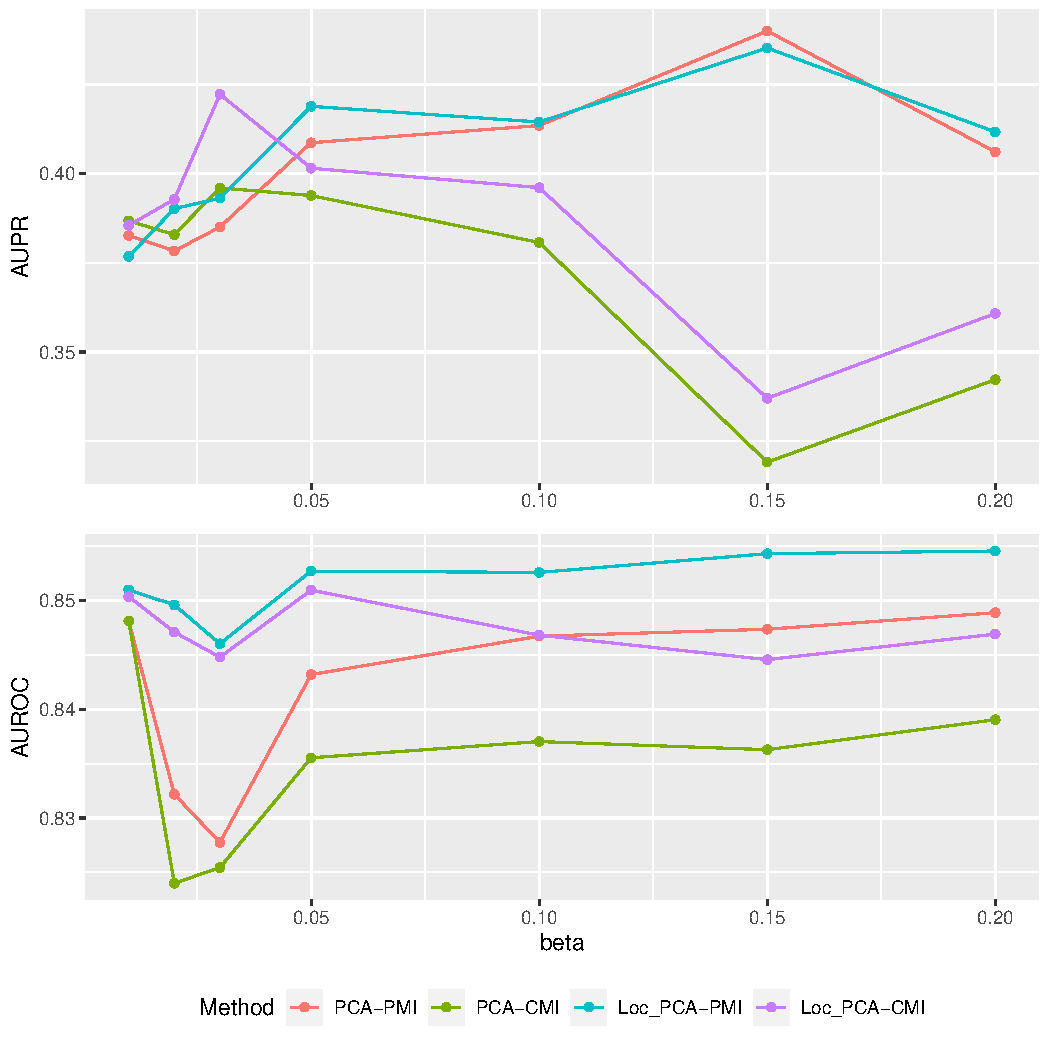
\includegraphics[width = \linewidth]{lamda_Dream50_Ecoli.pdf}}
      \centerline{(a) DREAM3-50 Ecoli}
      \medskip  
    \end{minipage}
    \begin{minipage}[b]{0.45\linewidth}
      \centering
      \centerline{
        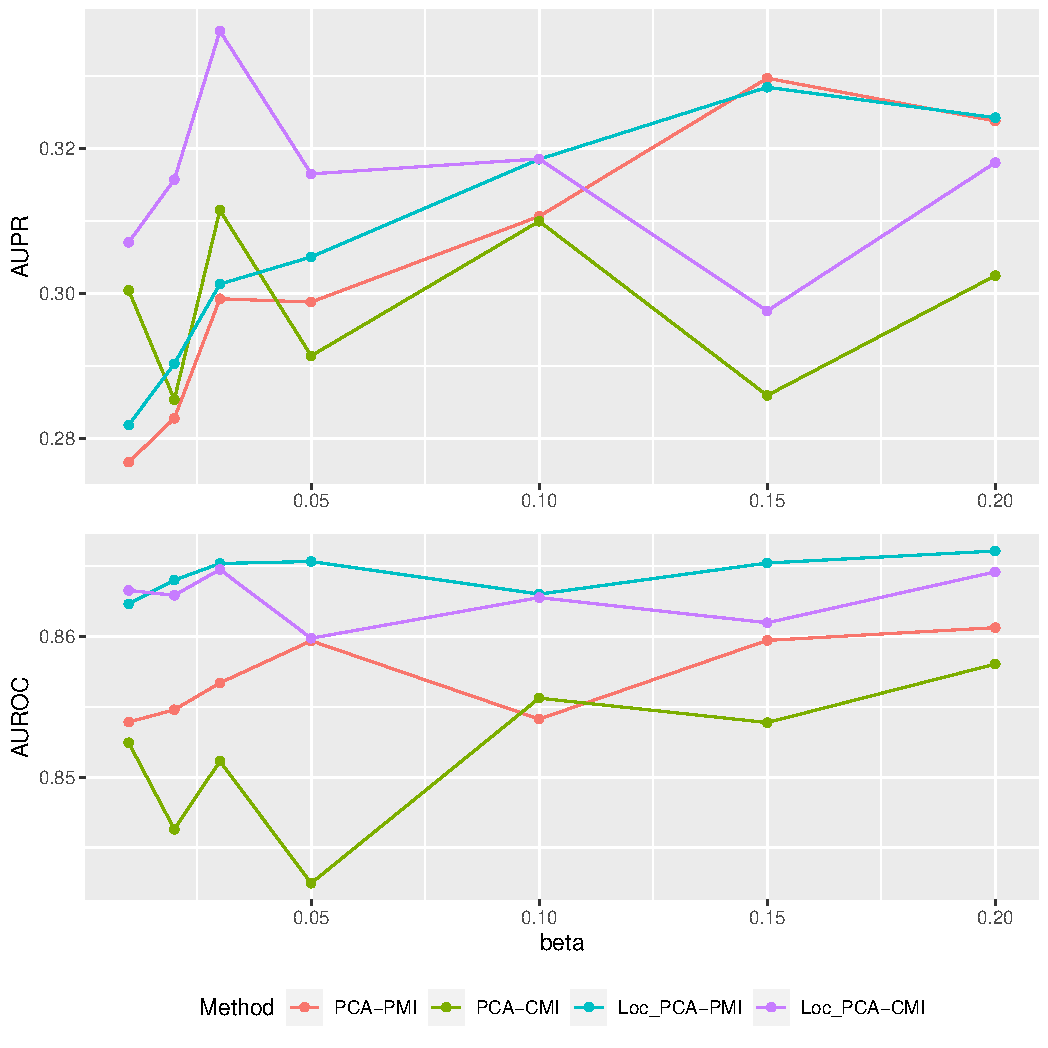
\includegraphics[width =\linewidth]{lamda_Dream100_Ecoli.pdf}}
      \centerline{(b) DREAM3-100 Ecoli}
      \medskip  
    \end{minipage}
      \begin{minipage}[b]{0.45\linewidth}
      \centering
      \centerline{
        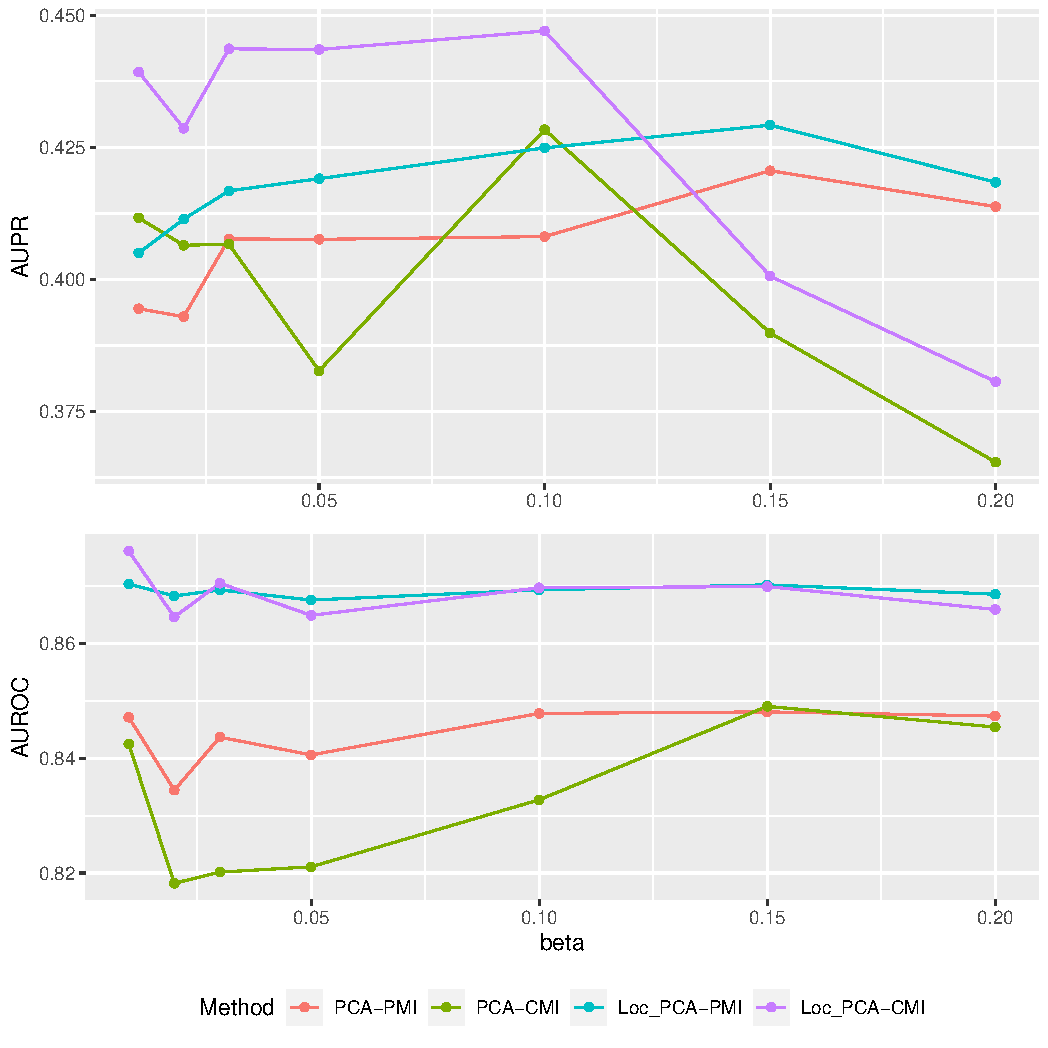
\includegraphics[width = \linewidth]{lamda_Dream50_Yeast.pdf}}
      \centerline{(c) DREAM3-50 Yeast}
      \medskip  
    \end{minipage}
    \begin{minipage}[b]{0.45\linewidth}
      \centering
      \centerline{
        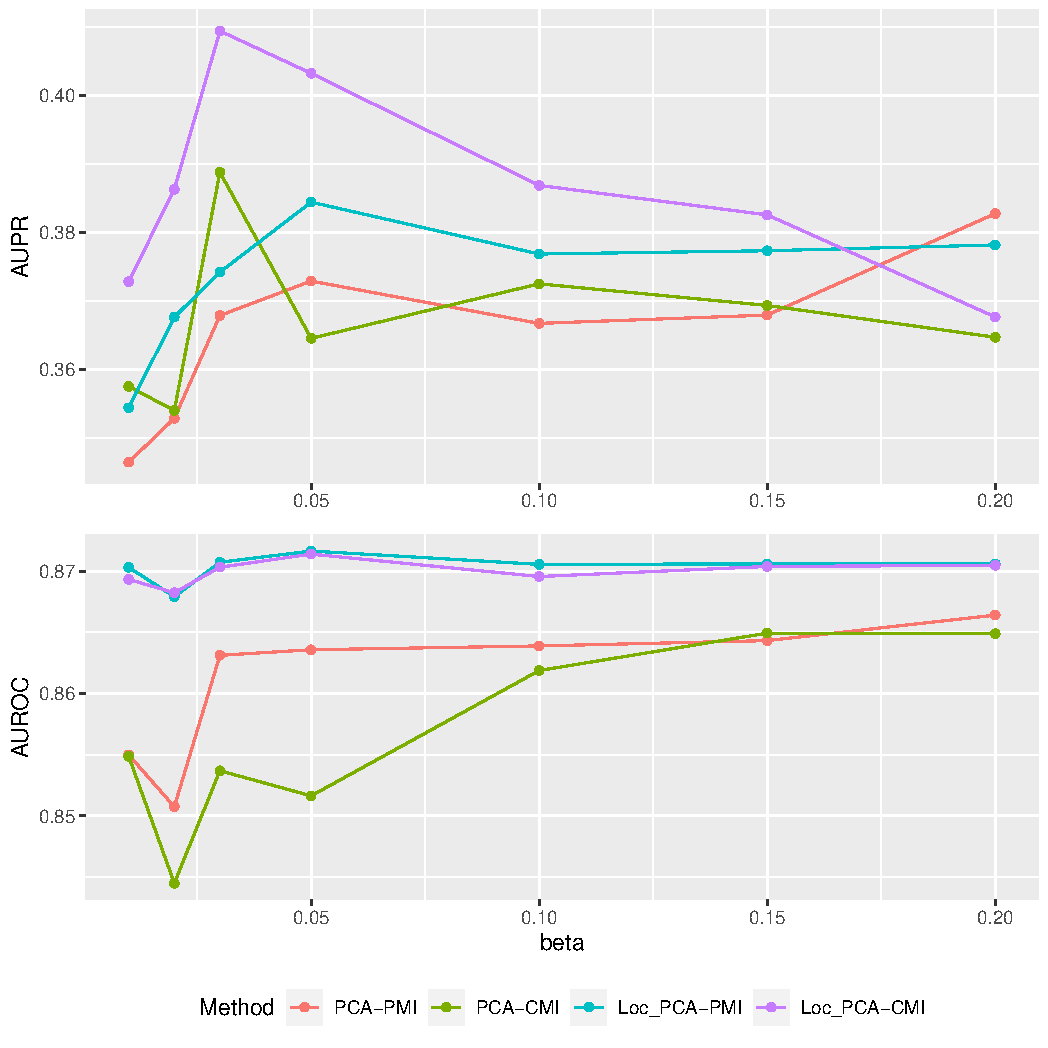
\includegraphics[width =\linewidth]{lamda_Dream100_Yeast.pdf}}
      \centerline{(d) DREAM3-100 Yeast}
      \medskip  
    \end{minipage}
    \caption{%AUPR and AUROC  by varying $k$ from 1 to 10 of four PCA based methods on four different datasets: 
    在四个不同的数据集上 $\beta$ 逐步改变, 基于路径一致性的四个算法的 AUPR 和 AUROC 结果示意图。
    }
    \label{fig:beta}
\end{figure*}

\subsubsection{实验结果分析}
%\subsubsection{局部结构策略的引入有效提升了 PCA-CMI 和 PCA-PMI 的性能}

相对于 PCA-CMI,  Loc-PCA-CMI 引入了
根据共表达的边进行局部基因聚类的策略,为了验证这个策略是否有效,我们对比了 Loc-PCA-CMI 和 PCA-CMI 在 AUPR 上的变化。
同理, 我们也对比了 Loc-PCA-PMI 和 PCA-PMI。
这四个算法的参数统一设置为: $\beta = 0.03$, $k = 2$。
结果如图 \ref{fig:loc} 所示,
在这四个不同的数据集上, Loc-PCA-CMI 和 Loc-PCA-PMI 分别比 PCA-CMI 和 PCA-PMI 具有更高的 AUPR 值,
可以看出局部聚类策略有助于提高 PCA-CMI 和 PCA-PMI 这两种方法的性能。

\begin{figure*}[!htbp]
  \centering
  \begin{minipage}[b]{0.45\linewidth}
    \centering
    \centerline{
      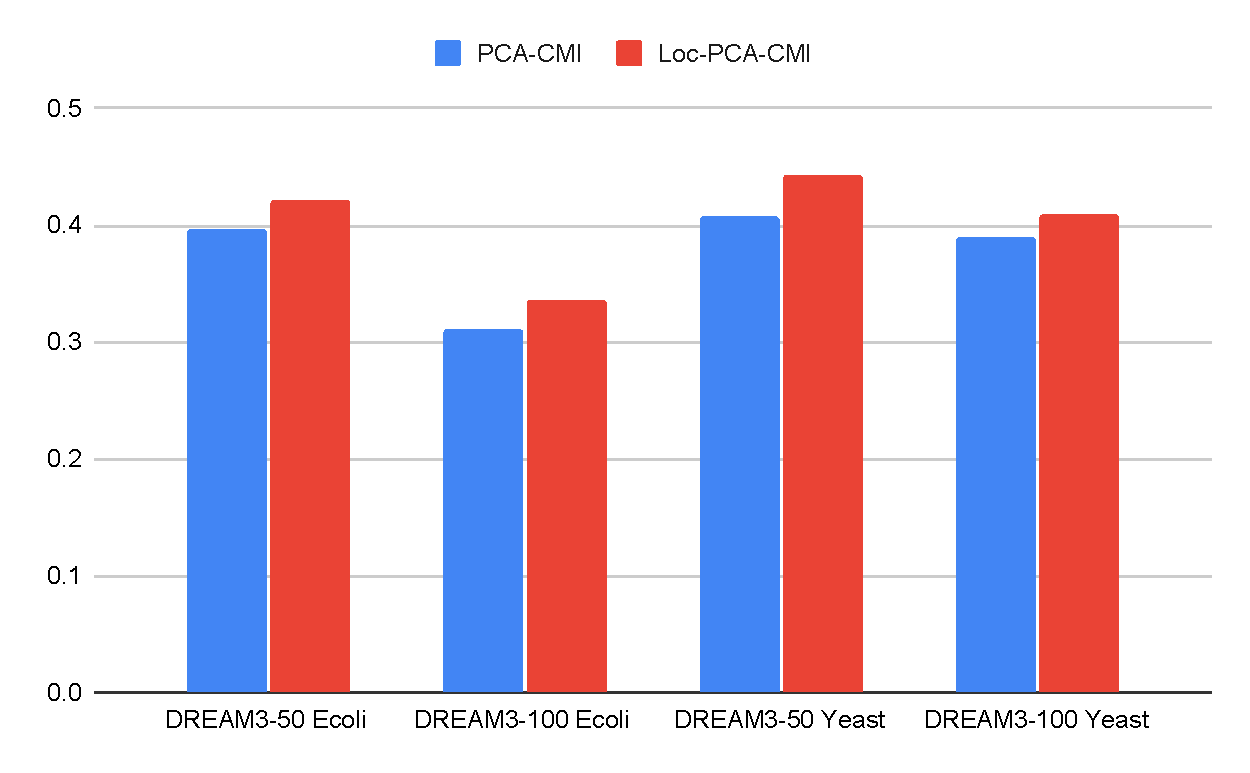
\includegraphics[width = \linewidth]{chart_loc_pcacmi_aupr.pdf}}
    \centerline{(a) Loc-PCA-CMI 和 PCA-CMI}
    \medskip  
  \end{minipage}
  \begin{minipage}[b]{0.45\linewidth}
    \centering
    \centerline{
      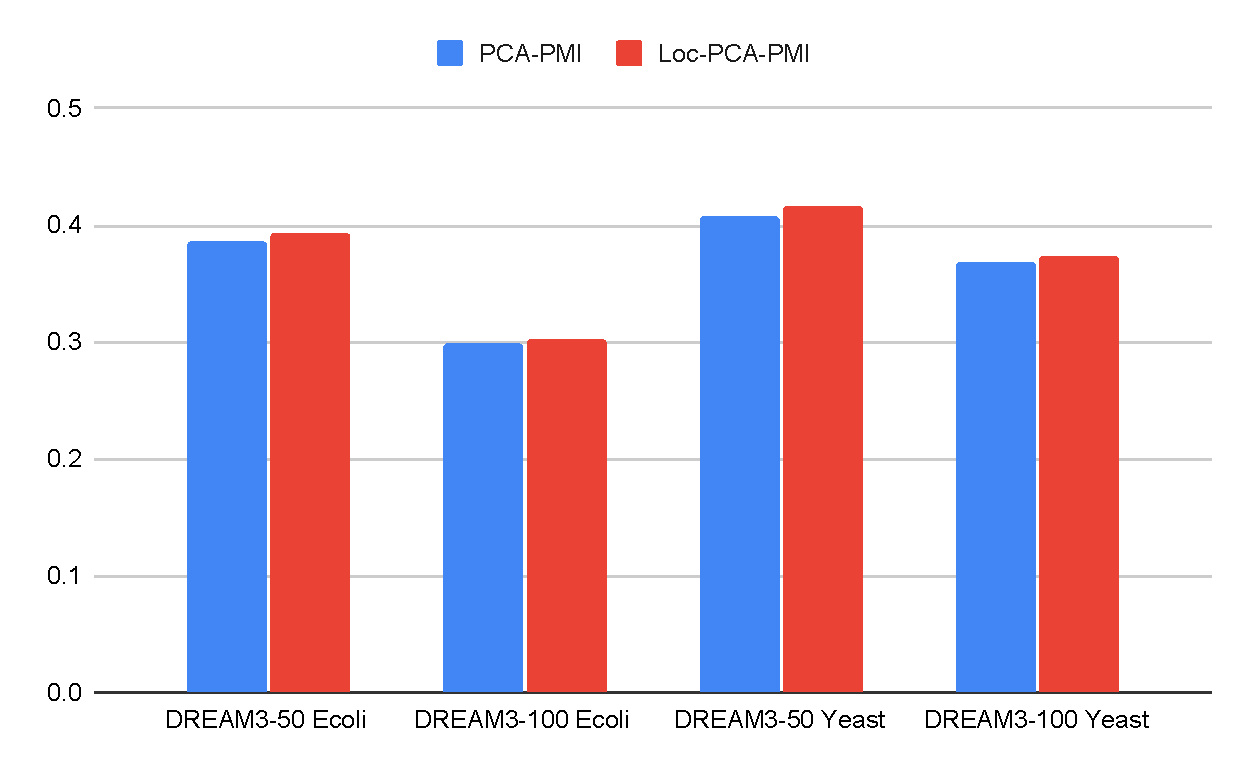
\includegraphics[width =\linewidth]{chart_loc_pcapmi_aupr.pdf}}
    \centerline{(b) Loc-PCA-PMI 和 PCA-PMI}
    \medskip  
  \end{minipage}
    
  \caption{
    局部结构策略的引入提升了 PCA-CMI 和 PCA-PMI 的性能。
  }
  \label{fig:loc}
\end{figure*}

% \subsubsection{Loc-PCA-CMI 比其它竞争方法表现更好}
我们在六个基准数据集上使用 Loc-PCA-CMI 和四种方法 ARACNE、MRNET、PCA-PMI、PCA-CMI 进行了比较实验。
我们使用 R 包 ``minet"和其默认参数来评估 ARACNE 和 MRNET,
采用了 Pearson 相关性系数直接从连续基因敲除表达数据中近似估计这两个方法中涉及到的 MI 矩阵 \upcite{olsen2008impact,meyer2010information} 。
为了评估 PCA-PMI 和 PCA-CMI, 我们根据对应的文献 \upcite{zhang2011inferring,zhao2016part} 中提供的 URL 下载了 MATLAB 代码。
另外, PCA-PMI 和 PCA-CMI 方法中的参数使用它们推荐的默认值,也就是 $\beta = 0.03$ 和 $k = 2$。
对于 Loc-PCA-CMI, 我们还对这两个参数采用了相同的值进行比较。
表 \ref{tab:performance_comparison} 给出了实验结果的 AUROC 和 AUPR。
从表中可以看出,当网络规模增大时,所有的方法的 AUPR 都会急剧下降。
Loc-PCA-CMI 仅在 DREAM3-10 Yeast 数据集中的 PCA-PMI (或本章提出的 Loc-PCA-PMI )之后,
而在其它五个数据集中,就 AUROC 和 AUPR 而言,
Loc-PCA-CMI 表现优于 ARACNE、MRNET、PCA-PMI 和 PCA-CMI 这四种方法。
此外,为了更完整地比较,我们还在表中展示了 Loc-PCA-PMI 的实验结果,
其中 $\beta = 0.03$ 和 $k = 2$。
Loc-PCA-CMI 和 Loc-PCA-PMI 在 AUROC 上几乎相同。
然而,在大多数数据集中, Loc-PCA-CMI 的 AUPR 优于 Loc-PCA-PMI。
所有方法、基准数据集和测评脚本相关的资料公开在 GitHub 仓库 \url{https://github.com/chenxofhit/Loc-PCA-CMI.git} 上。

\begin{table}[!htbp]
  %\caption{AUROC and AUPR for the six datasets using different methods}  
  \caption{使用不同方法在六个数据集上的 AUROC 和 AUPR 结果}  
  \label{tab:performance_comparison} 
    % \scalebox{0.9}{
    % \begin{minipage}{1.1\linewidth}
    \resizebox{\columnwidth}{!}{%
      \centering  
      \begin{threeparttable}  
        \begin{tabular}{ccccccccccccc}  
        \toprule  
        \multirow{2}{*}{Dataset}&  
        \multicolumn{2}{c}{ARACNE}&\multicolumn{2}{c}{MRNET}&\multicolumn{2}{c}{PCA-PMI}&\multicolumn{2}{c}{Loc-PCA-PMI}&\multicolumn{2}{c}{PCA-CMI}&\multicolumn{2}{c}{Loc-PCA-CMI}\\
        \cmidrule(lr){2-3} \cmidrule(lr){4-5}  \cmidrule(lr){6-7}  \cmidrule(lr){8-9}  \cmidrule(lr){10-11}  \cmidrule(lr){12-13} 
        &AUROC&AUPR &AUROC&AUPR &AUROC&AUPR &AUROC&AUPR &AUROC&AUPR &AUROC&AUPR\\
        \midrule  
        DREAM3-10 Ecoli  & 0.523 &0.255   &0.518&0.258    &0.816&0.483    &0.816&0.483    &{0.825}&{0.499}   &\textbf{0.825}&\textbf{0.499}\\
        DREAM3-50 Ecoli  &0.474 &0.050    &0.529&0.061    &0.828&0.385    &\textbf{0.846}&0.393    &0.825&0.396 &0.845&\textbf{0.422}\\
        DREAM3-100 Ecoli &0.505&0.027     &0.488&0.025    &0.857&0.299    &0.865&0.301    &0.851&0.311       &\textbf{0.865}&\textbf{0.336}\\
    
        DREAM3-10 Yeast  &0.628&0.321     &0.644&0.322    &0.995&0.933    &\textbf{0.995}&\textbf{0.933} &0.993&0.918 &0.993&0.918\\
        DREAM3-50 Yeast  &0.507&0.074     &0.524&0.080    &0.844&0.408    &0.869&0.417 &0.820&0.406   &\textbf{0.871}&\textbf{0.444}\\
        DREAM3-100 Yeast &0.547&0.040     &0.556&0.042    &0.863&0.368    &\textbf{0.871}&0.374 &0.854&0.389   &0.870&\textbf{0.409}\\
        \bottomrule  
        \end{tabular}  
        \end{threeparttable}  
        %   \end{minipage}
        %   }
        }
\end{table} 

\subsection{小结}

本章中,我们按照推断局部基因调控网络结构,然后不断合并局部结构来构造全局网络的策略,
提出了一种基于互信息和局部结构融合的 GRN 结构推断方法 Loc-PCA-CMI。
与 PCA 类算法 top-down 的思想相反, Loc-PCA-CMI 采用了类似 bottom-up 的策略。
在 DREAM3 敲除数据集上的实验表明, Loc-PCA-CMI 受益于局部聚类的策略。
此外, Loc-PCA-CMI 优于其它方法,
包括 ARACNE、MRNET、PCA-PMI 和 PCA-CMI,
特别是在大小为 50 和 100 的网络上 Loc-PCA-CMI 的表现更佳。

Loc-PCA-CMI 在处理局部网络结构的时候引入了 PCA-CMI,因此其计算效率也会受到 PCA-CMI 的影响,
特别是在处理大型数据集时。
因为在大型网络的情况下,局部基因簇的数量可能会非常大。
但是,如果可以控制每个局部簇的大小,本章提出的方法 Loc-PCA-CMI 也适用于大型的数据集上进行基因调控网络的构建。
我们未来的工作之一是改进聚类策略,
例如整合蛋白质复合物 \upcite{li2017identification,li2017dynetviewer},
以便更有效地处理大规模的基因表达数据。
另外,值得注意的是,我们主要关注推断 GRN 的结构,并没有考虑网络自身的稳定性问题。
因此,在未来的研究中我们将尝试从网络稳定性的角度出发,来推断更鲁棒的基因调控网络结构。

